\newcommand{\nTheo}{92}
\newcommand{\nMeth}{221}
\newcommand{\nEmp}{526}

To assess the past empirical and theoretical literature on psychological
acculturation, we performed a systematic review. We first read seminal
and review works within the field
\citep[including,][]{Ward2019, Berry1997b, Berry2003, Szapocznik1978, Sam2006a, Rudmin2003a}.
Based on our reading of the literature, we designed a comprehensive
literature search strategy in an iterative fashion. For the empirical
work on acculturation we performed a literature search on March
4\textsuperscript{th}, 2020 and February 14\textsuperscript{th}, 2021,
within the ``APA PsycINFO'' bibliographic databases using the
EBSCO\textit{host} provider. The databases also included the
PsycARTICLES, PsycBOOKS, and PsycCRITIQUES databases as well ProQuest
Dissertations with psychological relevance (for the full information on
the search strategy see Appendix \ref{app:AppendixSearchStrategy}).
\Warning~Should We Discuss Search Terms in Main Text? \Warning

Together with past reviews, we used this literature search to identify
validated scales as well as empirical works more generally. For the
theoretical literature we collected the theories used in the empirical
works and performed an additional, more specific, search of the same
databases as well as the Web of Science Core Collection using the
Clarivate Analytics provider on March 3\textsuperscript{rd}, 2021 (for
full information see Appendix \ref{app:AppendixSearchStrategy}).
\Warning~Should We Discuss Search Terms in Main Text? \Warning~

From the literature searches we created three separate databases of
theoretical, methodological, and applied empirical works on
psychological acculturation. For each literature search, we downloaded
all references and abstracts, which two independent coders screened for
relevance after duplicate removal --- first based on the titles and then
based on the abstracts. We downloaded all relevant and available works
for full-text coding. For all three types of works we extracted a range
of variables to apply our framework. The full coding process and data
extraction is described in the online Supplemental Information \hl{B}
(as well as on
\hl{citation to public OSF and/or GitHub repository goes here}).

\subsection{Theoretical Literature}

The most abstract level of our review was concerned with how researchers
conceptualized psychological acculturation in their theoretical work.
Our theory-specific literature search produced a total of 477 results
from which we identified 73 theories. From our review of the empirical
literature we added an additional 19 theories (total N = 92, for
exclusion reasons see Table \ref{tab:ExclusionsCombined} and for our
PRISMA diagram see Figure \ref{fig:PRISMA_Theories}. A full table of all
theories, with references, and final coding is available in our online
supplementary information as well as on our open science repository
(\hl{OSF and/or GitHub citation here}).

\begin{figure}[h]
\centering
\caption{PRISMA Diagram Theoretical Literature. Currently generated in R based on n(row) maybe make prettier.}
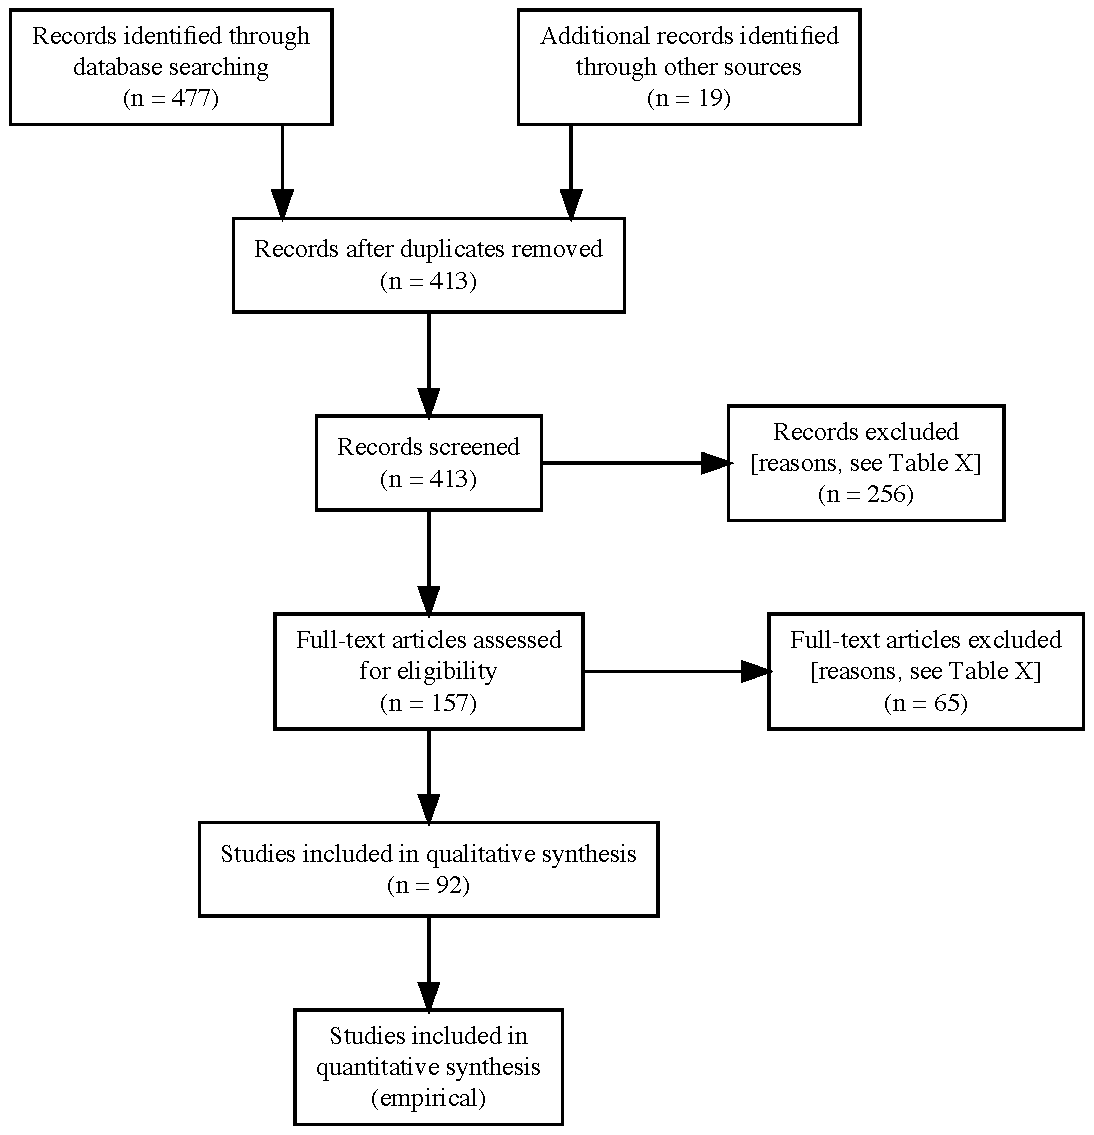
\includegraphics[width=\textwidth]{Figures/PRISMA_Theories}
\label{fig:PRISMA_Theories}
\end{figure}

\begin{table}
\begin{minipage}[t][\textheight][t]{\textwidth}

\caption{\label{tab:ExclusionsCombined}Exclusion Reasons for all Literature Levels}
\begin{tabular}[t]{lccccccc}
\toprule
\multicolumn{1}{c}{ } & \multicolumn{3}{c}{Theoretical} & \multicolumn{1}{c}{Psychometric} & \multicolumn{3}{c}{Empirical} \\
\cmidrule(l{3pt}r{3pt}){2-4} \cmidrule(l{3pt}r{3pt}){5-5} \cmidrule(l{3pt}r{3pt}){6-8}
Reason & Title & Abstract & Full Text & Full Text & Title & Abstract & Full Text\\
\midrule
not English & 5 & 1 & 1 & 1 & 1 &  & \\
not migration & 45 & 3 & 1 &  & 62 & 42 & 7\\
not migrant & 24 & 11 & 4 & 1 & 65 & 41 & 6\\
not acculturation & 49 & 17 & 16 & 1 & 225 & 116 & 12\\
not ABCD & 7 & 1 &  &  & 29 & 42 & 5\\
not theory & 20 & 71 & 25 &  &  &  & \\
not measured &  &  &  & 1 &  & 32 & 35\\
items not accessible &  &  &  & 16 &  &  & 36\\
thesis not accessible &  & 1 &  & 1 &  &  & 33\\
article not accessible &  &  &  & 1 &  &  & 4\\
book not accessible &  &  &  &  &  &  & 4\\
chapter not accessible &  &  &  & 1 &  &  & 2\\
poster not accessible &  & 1 &  &  &  &  & \\
\bottomrule
\end{tabular}
\end{minipage}
\end{table}


\subsubsection{Methods}
\paragraph{Dataset}

The authors of the 92 included theoretical works self-categorized their
contributions as a theoretical conceptualization (\textit{N} = 9),
theoretical framework (\textit{N} = 26), theory (\textit{N} = 36), or
theoretical model (\textit{N} = 21). And while 29 authors explicitly
targeted a specific part of acculturation (e.g., 7 identity
acculturation theories and 4 labor market acculturation theories), a
majority of theoretical works offered commentary on the overall
construct of acculturation (N = 63). Looking at the types of theory
building, a majority of proposal were purely theoretical (N = 74) with
the remaining theoretical works growing out of qualitative
investigations (such as grounded theory approaches; N = 17).

\paragraph{Experience Aspects}

To assess the experience aspects that were considered as part of the
theoretical works, two independent coders coded the authors' axioms,
theorems, and model elements for self-identified inclusions of affects,
behaviors, and cognitions (Cohen's \(\varkappa\) = \hl{X.XX} (pooled and
individual?)). We only coded explicit mentions by the authors and we did
so on three different levels. An example of these three levels for
affect would be phrases of ``mood'' or ``emotions'' (construct level),
``anxiety'' or ``pride'' (concept level), and ``the migrant feels
\ldots{}'' (operationalization level). A list with further examples can
be found in Table \ref{tab:AspectExamples}.

\paragraph{Process}

To assess the focus on psychological acculturation as a process or an
outcome, we coded whether authors self-identified the theory as a
process (e.g., `process,' `development,' `longitudinal,' `temporal,'
`dynamic') or an outcome (e.g., `static,' `outcome,' `markers,'
`consequence').

\subsubsection{Results}

Our main goal was to assess the use of the four affect, behavior,
cognition, and desire elements within the theoretical conceptualizations
of psychological acculturation. Looking at the overall usage of the
experience aspects we find that virtually all theoretical works included
behavioral aspects (92.39\%; e.g., cultural practices, media
consumption) and a vast majority considered cognitive aspects (88.04\%;
e.g., navigation knowledge, ethnic identification). We found
considerably less mentions of affective (41.3\%; e.g., anxiety, pride)
and motivational aspects (39.13\%; e.g., independence goals, need to
belong). But the generally high usage of the aspects, also meant that
only about a tenth of the theories focused on a single aspect (10.87\%).
Interestingly, all theories that considered only one aspect were
exclusively focusing on behaviors (N = 7) or cognitions (N = 3). Of the
remaining theories, 20 (i.e., 21.74\%) considered all four aspects,
leaving a majority of theoretical works to considered two aspects
(39.13\%) or three aspects (28.26\%). Among these, the most common
combinations of experience aspects were behavioral and cognitive
acculturation (30.43\%) or behavioral, cognitive, and motivational
aspects combined (15.22\%; also see Figure \ref{fig:ElementsTheories}
and Table \ref{tab:CombinedCooccurrences}).

Looking at the number of aspects considered together we also see
substantial differences in what kind of theories include a certain
aspect. Theories that included behaviors considered an average of 1.69
other aspects (\textit{sd} = 0.86), and theories considering cognitions,
on average, also included 1.78 other aspects (\textit{sd} = 0.75).
Theories that included the more internal aspects of affect or desire
showed a considerably higher number of additional aspects considered
(affect: \textit{m} = 3.37, \textit{sd} = 0.56; desire: \textit{m} =
3.50, \textit{sd} = 0.37). Thus, most scales measure multiple dimensions
(\textit{m} = 2.61, '\textit{sd} = 0.90; also see Figure
\ref{fig:CombinedAspectComplexity}). Yet they tend to focus on more
external aspects of behavioral and cognitive acculturation, and less on
internal aspects of affects and desires. This is also visible in the
observation that there were no theories that exclusively focused on
emotional or motivational acculturation while this was the case for both
cognitions and behaviors. And if emotional or desire aspects were
considered they were found in theories that tended to already include a
higher number of other experience aspects.

\begin{figure}[h]
\centering
\caption{Theories: Bar graph of the experience element combinations.}
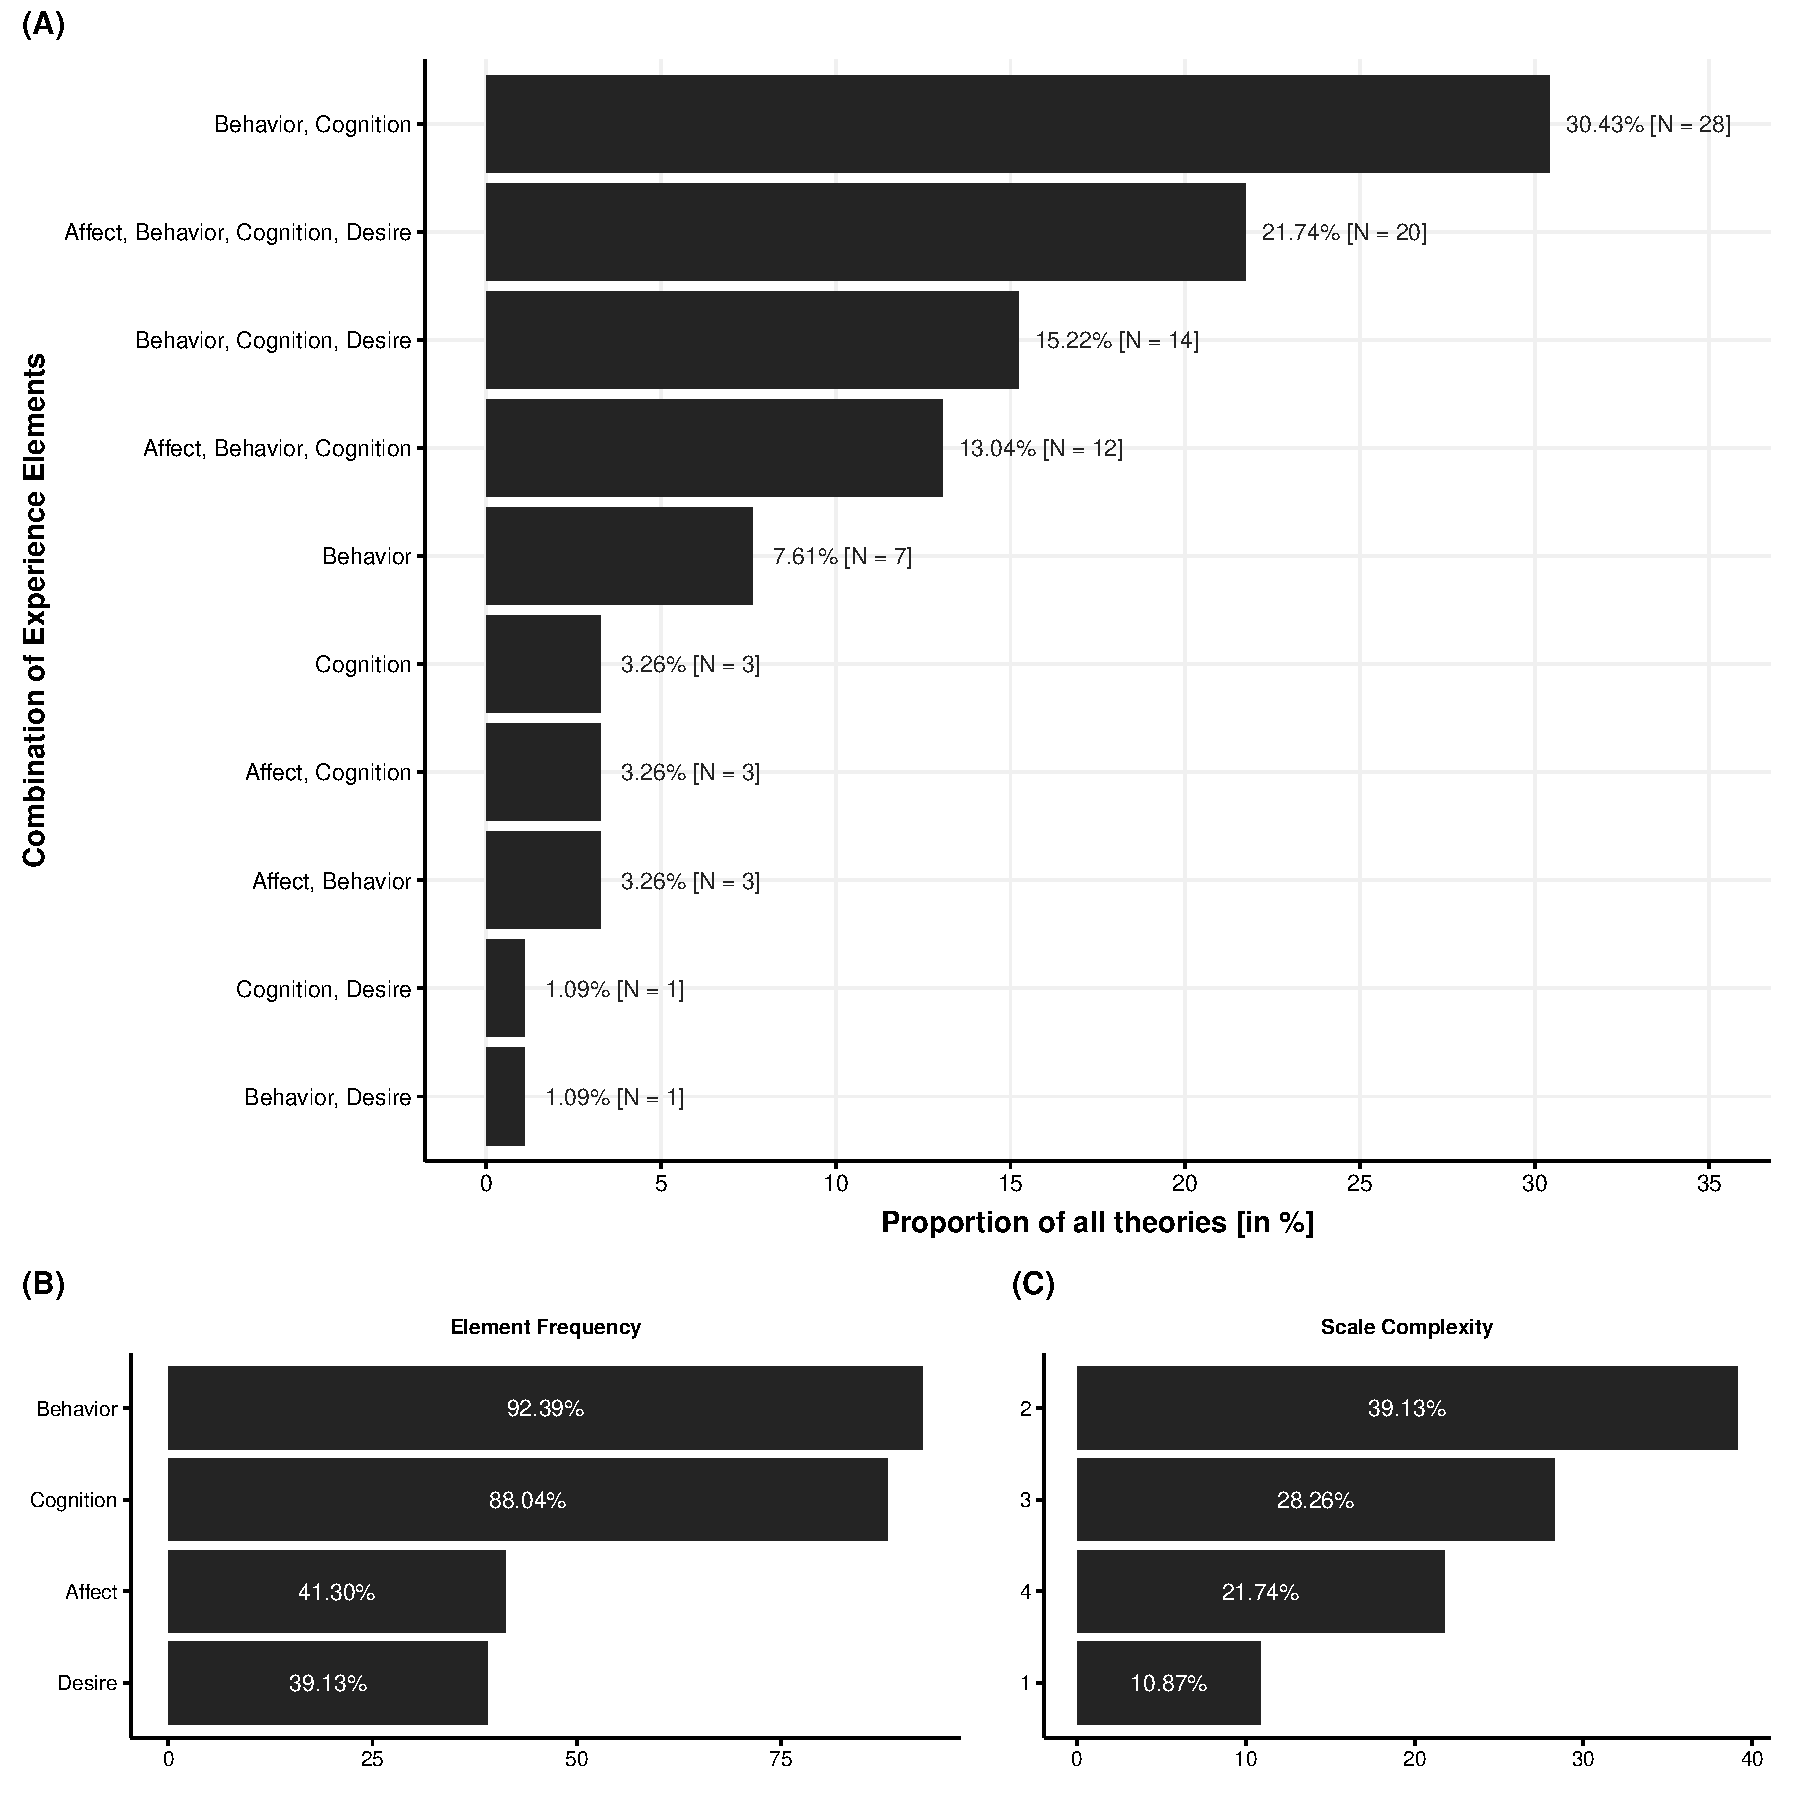
\includegraphics[width=\textwidth]{Figures/TheoriesFreq-1}
\label{fig:ElementsTheories}
\end{figure}

\begin{table}
\begin{minipage}[t][\textheight][t]{\textwidth}

\caption{\label{tab:CombinedCooccurrences}Bivariate Asspociation of Aspects for all Literature Levels.}
\begin{tabular}[t]{lcccc}
\toprule
\multicolumn{1}{c}{Aspect} & Affect & Behavior & Cognition & Desire\\
\midrule
\addlinespace[0.3em]
\multicolumn{5}{l}{\textbf{Theoretical (\textit{N} = 92)}}\\
\hspace{1em}Affect & \textit{N} = 38 & -0.01 & 0.11 & 0.23*\\
\hspace{1em}Behavior & 35 & \textit{N} = 85 & -0.11 & 0.15\\
\hspace{1em}Cognition & 35 & 74 & \textit{N} = 81 & 0.23*\\
\hspace{1em}Desire & 20 & 35 & 35 & \textit{N} = 36\\
\addlinespace[0.3em]
\multicolumn{5}{l}{\textbf{Methodological (\textit{N} = 233)}}\\
\hspace{1em}Affect & \textit{N} = 117 & -0.05 & 0.22*** & 0.22***\\
\hspace{1em}Behavior & 83 & \textit{N} = 170 & -0.08 & -0.10\\
\hspace{1em}Cognition & 111 & 146 & \textit{N} = 204 & 0.16*\\
\hspace{1em}Desire & 46 & 45 & 65 & \textit{N} = 68\\
\addlinespace[0.3em]
\multicolumn{5}{l}{\textbf{Empirical (\textit{N} = 526)}}\\
\hspace{1em}Affect & \textit{N} = 259 & 0.03 & 0.29*** & 0.09*\\
\hspace{1em}Behavior & 210 & \textit{N} = 421 & -0.10* & -0.02\\
\hspace{1em}Cognition & 241 & 336 & \textit{N} = 430 & 0.09\\
\hspace{1em}Desire & 57 & 76 & 86 & \textit{N} = 97\\
\bottomrule
\multicolumn{5}{l}{\rule{0pt}{1em}\textit{Note: }}\\
\multicolumn{5}{l}{\rule{0pt}{1em}Diagonal: Times aspect occurred;}\\
\multicolumn{5}{l}{\rule{0pt}{1em}Upper triangle: Phi association;}\\
\multicolumn{5}{l}{\rule{0pt}{1em}Lower triangle: Times aspects co-occurred.}\\
\end{tabular}
\end{minipage}
\end{table}


\subsection{Methodological Literature}

Based on the systematic review and its coding, the first empirical
dataset we assess is a database of scale validations. We bring together
the scales suggested in previous reviews as well as validation studies
we identified in our own review. Throughout our literature review we
found five major works that reviewed the measurement of acculturation
\citep{Celenk2011, Maestas2000, Matsudaira2006, Wallace2010, Zane2004}.
After removal of duplicate scales, we added any scale validation that
was present in our own systematic review but not included in the
previous reviews. For each measure we extracted the full item list as
well as the item scoring prior to coding. A comprehensive and
interactive database of the scales, with reference- and publication
information, as well as our experience elements and -context coding is
available in our online supplementary information as well as on our open
science repository (\hl{OSF and/or GitHub citation here}).

\subsubsection{Methods}  
\paragraph{Dataset}

Taken together these five reviews collected a total of 97 scales. From
our own review we added 151 additional validation studies. After
removing duplicates this meant that we considered a total of 247 unique
scales for our coding. Of these scales we ultimately had to exclude 23,
because they were either not accessible or did not fit the the topic of
our review (see Table \ref{tab:ExclusionsCombined}). About a quarter of
scales (24.29\%) included majority group members in their validation
studies. The earliest included validation was from 1948 with a majority
of scales being validated around the turn of the 21\textsuperscript{st}
century and the most recent included validation study was published in
2020.

\paragraph{Experience Aspects}

We extracted data on the experience aspects by primarily focusing on the
measured concepts and their operationalizations (also see Table
\ref{tab:AspectExamples}). For each article we retrieved the items used
and coded whether the measure included references to affects, behaviors,
cognitions, and desires. Because this concerned the most central aspect
of our framework, each manuscript was double-coded and inconsistent
codes were resolved after discussion (Cohen's \(\varkappa\) = \hl{X.XX}
(pooled and individual?)).

At this stage we also noted if items measured concepts that are complex
and relate to multiple experience aspects. As an example, a single item
asking about `satisfaction with the new life' might include emotional
and cognitive elements. In this case, we code the manuscript as
measuring both emotions and cognitions, but note that these elements are
not measured independently. We also noted if the measures do not
consider an individual's experiences, such as reporting migration status
or length of residency.

\paragraph{Process}

To extract an indicator of whether the scales were aimed at
psychological acculturation as a process or an outcome, we collected
information on assessed migration times (e.g., pre-migration,
post-migration) and the the validation type (e.g., cross-sectional,
longitudinal).

\paragraph{Context}

We additionally coded a range of contextual variables, including the
type of sample collected (e.g., student, clinical), the life domain
targeted (e.g., school, family), the cultures considered (i.e., host and
migrant groups), the type of analysis conducted (e.g., correlation,
regression), the measurement type (e.g., continuous scale, categorical
classification), as well as the variable type of acculturation in the
analysis (e.g., predictor, dependent). Further information as well as
analyses of the contextual variables go beyond the scope of the
immediate framework validation and are thus only presented in
Supplementary Material A.

\subsubsection{Results}

With our main aim of examining the experience structure within the
scales, we examined whether scales included a specific experience
element but also examined the used elements in their complex
combinations. In terms of general inclusion of elements, most studies
included a measure of cognition (86.43\%) and behavior (75.57\%),
whereas only roughly half the studies included a measure of affect
(52.49\%) and only a fourth of the scales included a measure of desires
(23.98\%). However, only a minority of scales included only a single
aspect. There were only 14 scales that exclusively relied on cognitions
(6.33\%) and 20 scales that measured only behaviors (9.05\%). Yet,
inversely, there were also only 30 scales that measured all four aspects
(13.57\%). Most studies measured two (41.63\%) or three (28.05\%)
aspects. A majority of scales either measured behavioral and cognitive
aspects (25.79\%) or behavioral, cognitive, and affective elements
(21.27\%; also see Figure \ref{fig:ElementsScales} and Table
\ref{tab:CombinedCooccurrences}).

Looking at the number of aspects measured together we also see
substantial differences in what kind of scales include a certain aspect.
Scales that included cognitions also measured an average of 1.56 others
aspects (\textit{sd} = 0.71), scales measuring behavior, on average,
also included 1.57 other aspects (\textit{sd} = 0.71). Scales measuring
affect or desire measures included substantially more other aspects.
Scales that included affect measures also included 1.97 other aspects
(\textit{sd} = 0.61) and scales measuring desires even measured an
average of 2.42 other aspects per scale (\textit{sd} = 0.56; also see
Figure \ref{fig:CombinedAspectComplexity}). Thus, most scales measure
multiple dimensions (\textit{m} = 2.38, \textit{sd} = 0.85), yet they
focus on external accessible aspects of psychological acculturation
(i.e., behavior and cognition), less of what is considered `internal' or
`subjective' (i.e., affect and desires). And if affect or desire
elements are considered, they often only occur in scales that already
include a higher number of other aspects. This is further underscored by
the observation that there were only 3 scales that exclusively measured
emotional acculturation and not a single scale that exclusively focused
on motivational acculturation (while this was the case for both
cognitions and behaviors). And if emotional or desire aspects were
measured they were on average measured in scales that had already
included more experience aspects.

\begin{figure}[h]
\centering
\caption{Scales: Bar graph of the experience element combinations.}
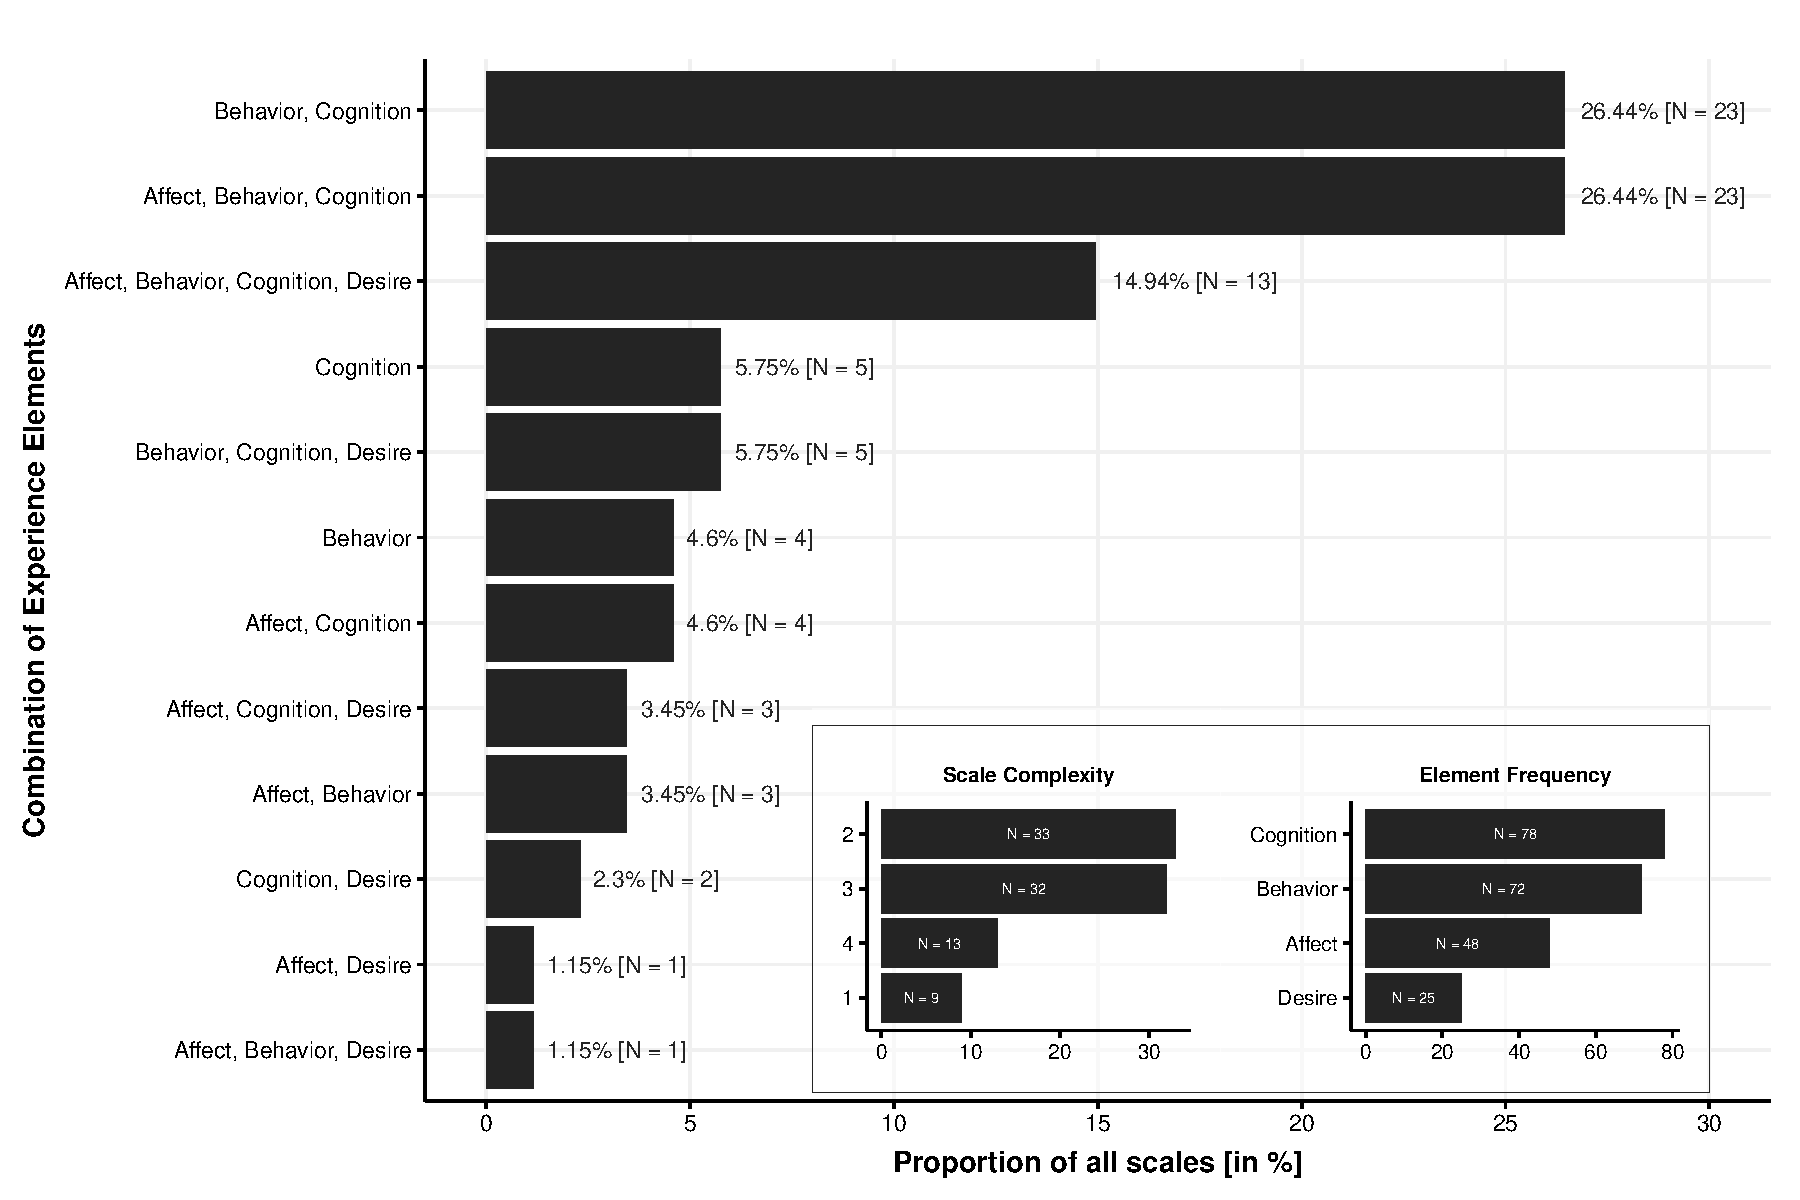
\includegraphics[width=\textwidth]{Figures/ABCDFreq-1}
\label{fig:ElementsScales}
\end{figure}

To assess the process focus of the scales we also assessed the migration
time the scale validators considered. Except for a single scale that was
validated for potential migrants, all scales were validated using
cross-sectional data after the migrant arrived in the settlement
society. This is in line with observations by previous reviews of the
field \citep[e.g.,][]{Brown2011}.

\subsection{Empirical Literature}

At the most applied level, we assessed the broader empirical studies.
This final database included the largest number of manuscripts and is in
theory the application of the theoretical and methodological literature.
The search produced a total of 1629 results to which we added 133
articles through contacts with experts in the field and from referenced
works within the review. We subsequently screened out results that did
not fit into our review. After duplicate removal (\(N_{excluded}\) =
300, \(N_{screened}\) = 1329), we excluded 383 results in the title
screening as well as an additional 272 results during the abstract
screening. Of the remaining 674 results, 666 papers presented empirical
work on acculturation and were coded. The 8 non-empirical results were
reviews, which were not coded because they did not measure cultural
adaptation. During the full text coding we excluded an additional 140
results because they were either not relevant or were not accessible
(for exclusion reasons see Table \ref{tab:ExclusionsCombined} and for
our PRISMA diagram see Figure \ref{fig:PRISMA}).

\begin{figure}[h]
\centering
\caption{PRISMA diagram. Position still undecided. Currently generated in R based on n(row) maybe make prettier.}
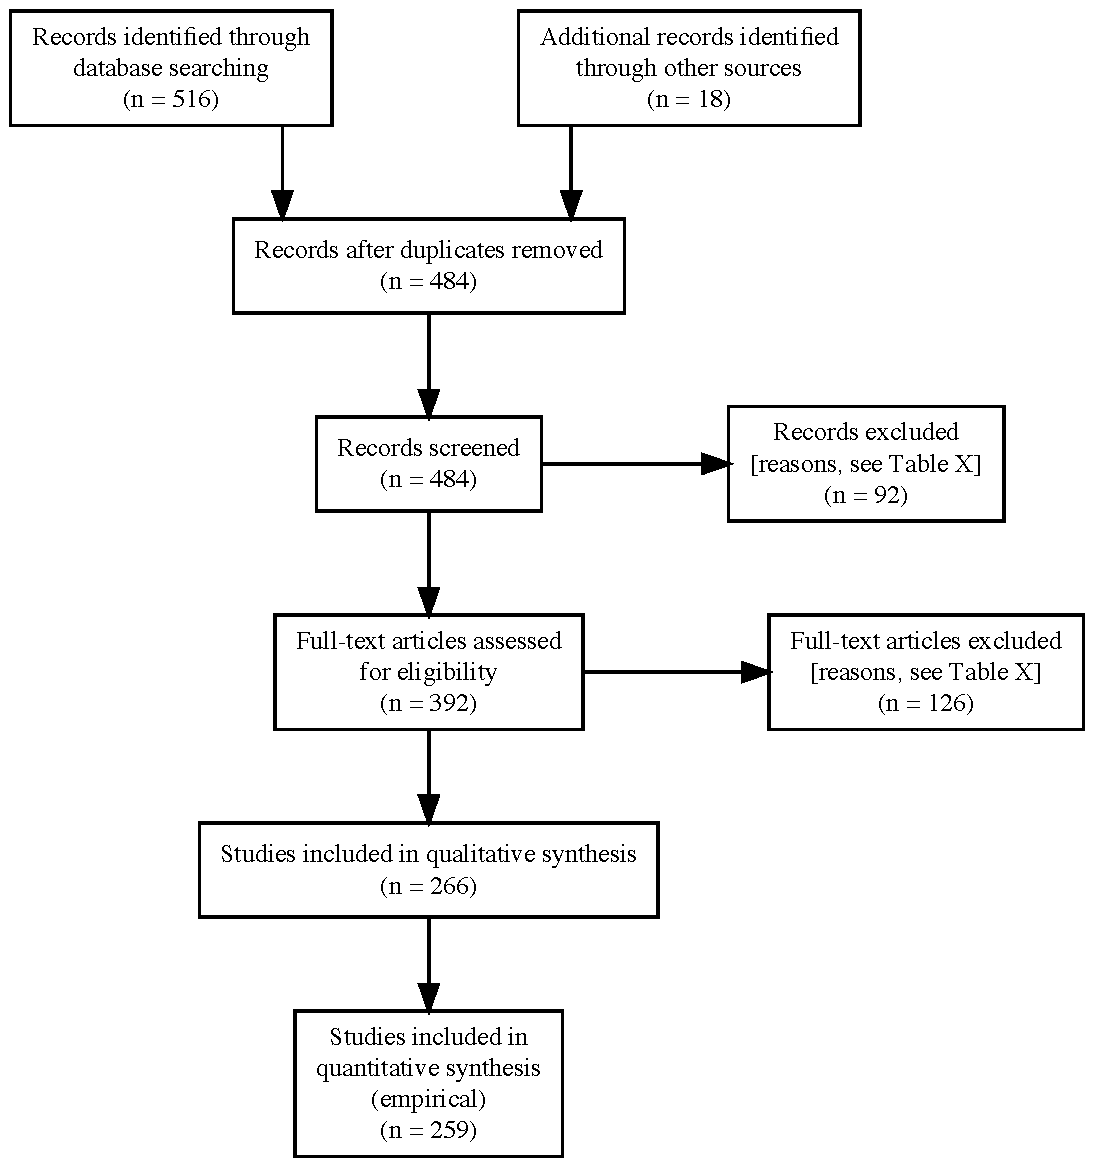
\includegraphics[width=\textwidth]{Figures/PRISMA}
\label{fig:PRISMA}
\end{figure}

\subsubsection{Methods}

\paragraph{Dataset}

Of the final works we coded, 452 were journal articles, 68 theses, and 6
book chapters. Most studies presented quantitative data (\textit{N} =
464), mixed methods (\textit{N} = 39), or qualitative data (\textit{N} =
20), while the remaining 3 manuscripts were reviews of empirical data.
Notably, a majority of the empirical investigations did not share common
measures of cultural adaptation -- 390 studies used measures that were
reported a maximum of five times, with a considerable majority of papers
using new or ad-hoc measures of cultural adaptation. Less than a fifth
of studies included the local majority in the study (\textit{N} = 77,
14.69\%). Cultural adaptation most frequently was a predictor variable
(\textit{N} = 285, 54.39\%), a dependent variable (\textit{N} = 148,
28.24\%), or a correlation variable (\textit{N} = 37, 7.06\%) in the
empirical works. This pattern was mirrored when looking at the focus of
the papers, where a majority of the papers had acculturation as their
main focus (\textit{N} = 153, 29.48\%), with other bodies of work
focusing on health outcomes (\textit{N} = 163, 31.41\%), or inter-group
relations (\textit{N} = 18, 3.47\%) as their main outcomes. The earliest
included study was published in 1948, with a strong increase of
publications after the year 2000, and a peak of publications in 2012. We
provide full descriptions of descriptive data extractions and additional
information about the data description in Online Supplementary
Information \hl{X}.

\paragraph{Experience Aspects}

Extraction of the used experience aspects mirrored the methodological
literature assessment and we primarily focused on the measured concepts
and their operationalizations (also see Table \ref{tab:AspectExamples}).
The only exception was qualitative studies, which we coded following the
same codebook of the theoretical literature. All aspects were coded by
two independent coders (Cohen's \(\varkappa\) = \hl{X.XX} (pooled and
individual?)) and inconsistencies were resolved after discussion.

\paragraph{Process}

To assess the static or dynamic conceptualization of the empirical
studies, we again collected information on assessed migration times
(e.g., pre-migration, post-migration) and additionally coded the type of
data collected and analyzed (e.g., cross-sectional, longitudinal data
and data analysis).

\paragraph{Context}

Contextual variables on sample, life domain, cultural groups,
measurement type, and variable type are again beyond the scope of the
framework validation but are presented in Supplementary Material A.

\paragraph{Field of Publication}

For the broader empirical literature, we also collected additional data
on the field the studies were published in. To that end, we merged the
`Scimago Journal Ranking Database' \citep{SCImago2020} with our
database. For all available journal articles we added information on key
journal metrics (incl.~H index, impact factor, and data on the field and
audiences). This also meant that dissertations, book chapters, and books
were excluded from this analysis because data on their publishers is not
readily available or unreliable. Additionally, 10 journals were not
included in the Scimago database (likely because they do not have an
ISSN identifier or were discontinued before 1996, see Online Appendix
\hl{X}, Table \hl{X} for the missing journals). We ultimately had
journal metrics for 437 empirical articles.

To summarize the journal data we then classified the journal fields into
super-ordinate discipline codes. These discipline codes are based in
part on U.S. Department of Education's subject classifications
\citep[i.e., CIP;][]{InstituteofEducationSciences2020}, the U.K.
academic coding system
\citep[JACS 3.0;][]{HigherEducationStatisticsAgency2013}, the Australian
and New Zealand Standard Research Classification
\citep[ANZSRC 2020;][]{AustralianBureauofStatistics2020}, as well as the
Fields of Knowledge project \citep{ThingsmadeThinkable2014}. We
ultimately classified each journal into one of four mutually exclusive
disciplines (psychology: \textit{N} = 131, multidisciplinary: \textit{N}
= 103, Medicine, Nursing, and Health: \textit{N} = 146, and Social
Sciences (miscellaneous): \textit{N} = 45. For a full discussion of the
classifications see Online Supplementary Materials \hl{X}).

\subsubsection{Results}

We assessed the role of experience aspects in the measurement and then
compared differences between fields.

In terms of the overall frequencies of experience elements, the broader
empirical data mirrored that of the validation studies. Most studies
included a measure of cognition (80.23\%) and behavior (82.32\%),
whereas only about half of all studies included a measure of affect
(49.05\%) and less than a fifth of the studies included a measure of
desires (17.11\%). Yet, only 118 studies focused on a single experience
aspect (\(N_{behavior\ only}\) = 75, \(N_{cognition\ only}\) = 38,
\(N_{emotion\ only}\) = 5). Similarly, only 42 papers included measures
of all four experience aspects (7.98\%). Most studies measured three
(35.17\%) or two aspects (34.41\%; (\textit{m} = 2.29, \textit{sd} =
0.81)). Different from the scale validations, within the broader
empirical works, most works included measures of emotions, behaviors,
and cognitions (\textit{N} = 154, 29.28\%), with a further substantial
number of articles measuring behaviors and cognitions (\textit{N} = 120,
22.81\%. Also see Figure \ref{fig:EmpPlotFreq-1} and Table
\ref{tab:CombinedCooccurrences}). Looking at the number of aspects
measured together we again see substantial differences in what kind of
scales include the individual aspects. Scales that included cognitions
measured an average of 1.54 other aspects (\textit{sd} = 0.63), scales
measuring behavior, on average, measured 1.43 other aspects (\textit{sd}
= 0.79), while scales that included affect measured an average of 1.93
other experience aspects (\textit{sd} = 0.43) and scales measuring
desires even measured an average of 2.28 other experience aspects
(\textit{sd} = 0.58; also see Figure
\ref{fig:CombinedAspectComplexity}). Thus, not a single study measured
only motivation (i.e., desires), and measures of desires remained mostly
limited to scales that were already measuring many of the other
experience aspects. The results exacerbate the pattern found in the
scale validations, complex measures and conceptions of acculturation are
seen infrequently and external aspects of cognition and behavior remain
the focus of most studies.

\begin{figure}[h]
\centering
\caption{Empirical Literature: Bar graph of the experience element combinations.}
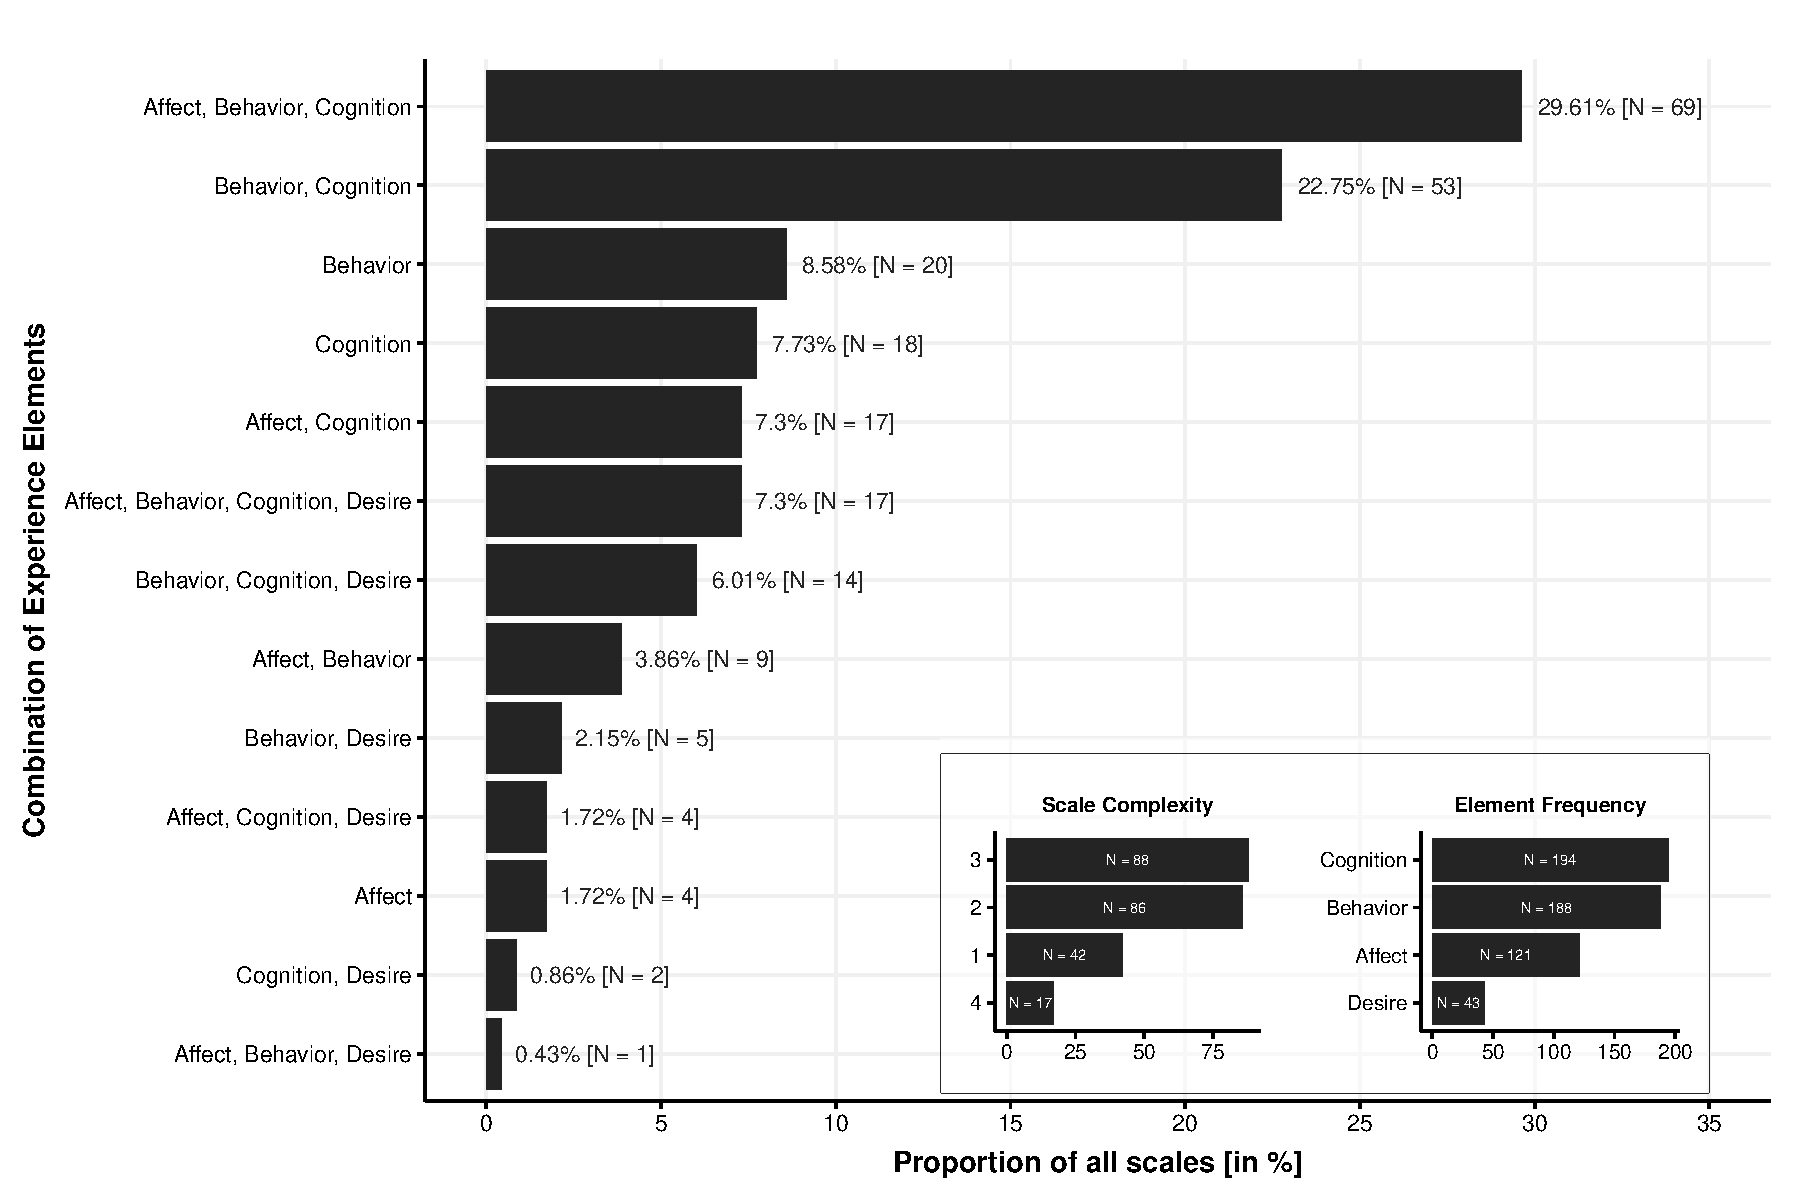
\includegraphics[width=\textwidth]{Figures/EmpPlotFreq-1}
\label{fig:EmpPlotFreq-1}
\end{figure}

To assess the process focus of the broader empirical works, we again
assessed when in the migration process the data was collected and we
additionally assessed the type analysis done by the authors. We found
that 512 studies (97.71\%) collected data after the arrival of the
migrant in the new society. Two studies targeted potential migrants and
10 studies collected data prior and following the migration event.
Moreover, only 25 studies included longitudinal data analyses of
psychological acculturation (4.79\%). This observation, again
underscores the arguments that the acculturation literature has thus far
failed to provide data that meaningfully captures migration as a process
\citep[e.g.,][]{Brown2011, Ward2019}.

To further assess the comparative utility of the experience framework,
we further assessed differences of experience aspects between academic
fields. For the full results, including differences in the methods, and
publication types as well as contextual differences in terms of sampling
procedures, situational domains, analyses, and cultural contexts see
Supplementary Online Material \hl{X}.

We first assessed the references to affect, behavior, cognition, and
desires separately, for each of the disciplines. We find that for all
fields desires (11.64-25.95\% of all measures in the field) and emotions
(37.67-58.78\%) are the least frequently measured elements and medical
journals measure them the least frequently (in proportional terms).
Looking at the common cognitive and behavioral elements the proportions
diverge between the fields. While the multidisciplinary field measured
behaviors (79.61\%) and cognition (79.61\%) almost equally often, in the
medical and general social science journals behaviors were measured
considerably more often than cognitions (\(Behavior_{SoSci}\) = 88.89\%
\textgreater{} \(Cognition_{SoSci}\) = 62.22\%; \(Behavior_{Med}\) =
88.36\% \textgreater{} \(Cognition_{Med}\) = 68.49\%). Inversely, in the
psychological journals cognitions (90.08\%) were measured more often
than behaviors (74.05\%; also see Figure \ref{fig:FieldPlotFreq} A and
B).

When looking at differences in how many different experience aspects
were measured together and patterns within these aspect-combinations,
differences between the fields become increasingly evident (also see
Figure \ref{fig:FieldPlotFreq} A and C). While `affect, behavior, and
cognition' and `behavior, and cognition' measures are common
combinations across all fields, there is less experience complexity and
variation for medical and social science fields. There were
statistically significant mean differences between the fields in terms
of how many experience aspects were considered (parametric:
\textit{F}(3, 421) = 6.39, \textit{p} = 0, non-parametric:
\textit{Kruskal-Wallis} \(\chi^{2}\) = 19.26, \textit{df} = 3,
\textit{p} = \textless.001, \(\eta_{p}^{2}\) = 0.04, 95\%CI{[}0.01,
0.08{]}). Looking at the mean differences in more detail, empirical
works published in psychological journals had significantly higher
average aspect counts (\textit{M} = 2.49, \textit{SD} = 0.74) than the
medical (\textit{M} = 2.06, \textit{SD} = 0.84) and the general social
science journals (\textit{M} = 2.02, \textit{SD} = 0.75; also see Figure
\ref{fig:FieldPlotComplexityAverage}). The broader patterns described
here thus point to heterogeneity between fields and show that different
fields diverge in the number and types of acculturation aspects they
tend to consider.

\begin{figure}[h]
\centering
\caption{Scale Complexity and their proportional occurences per field.}
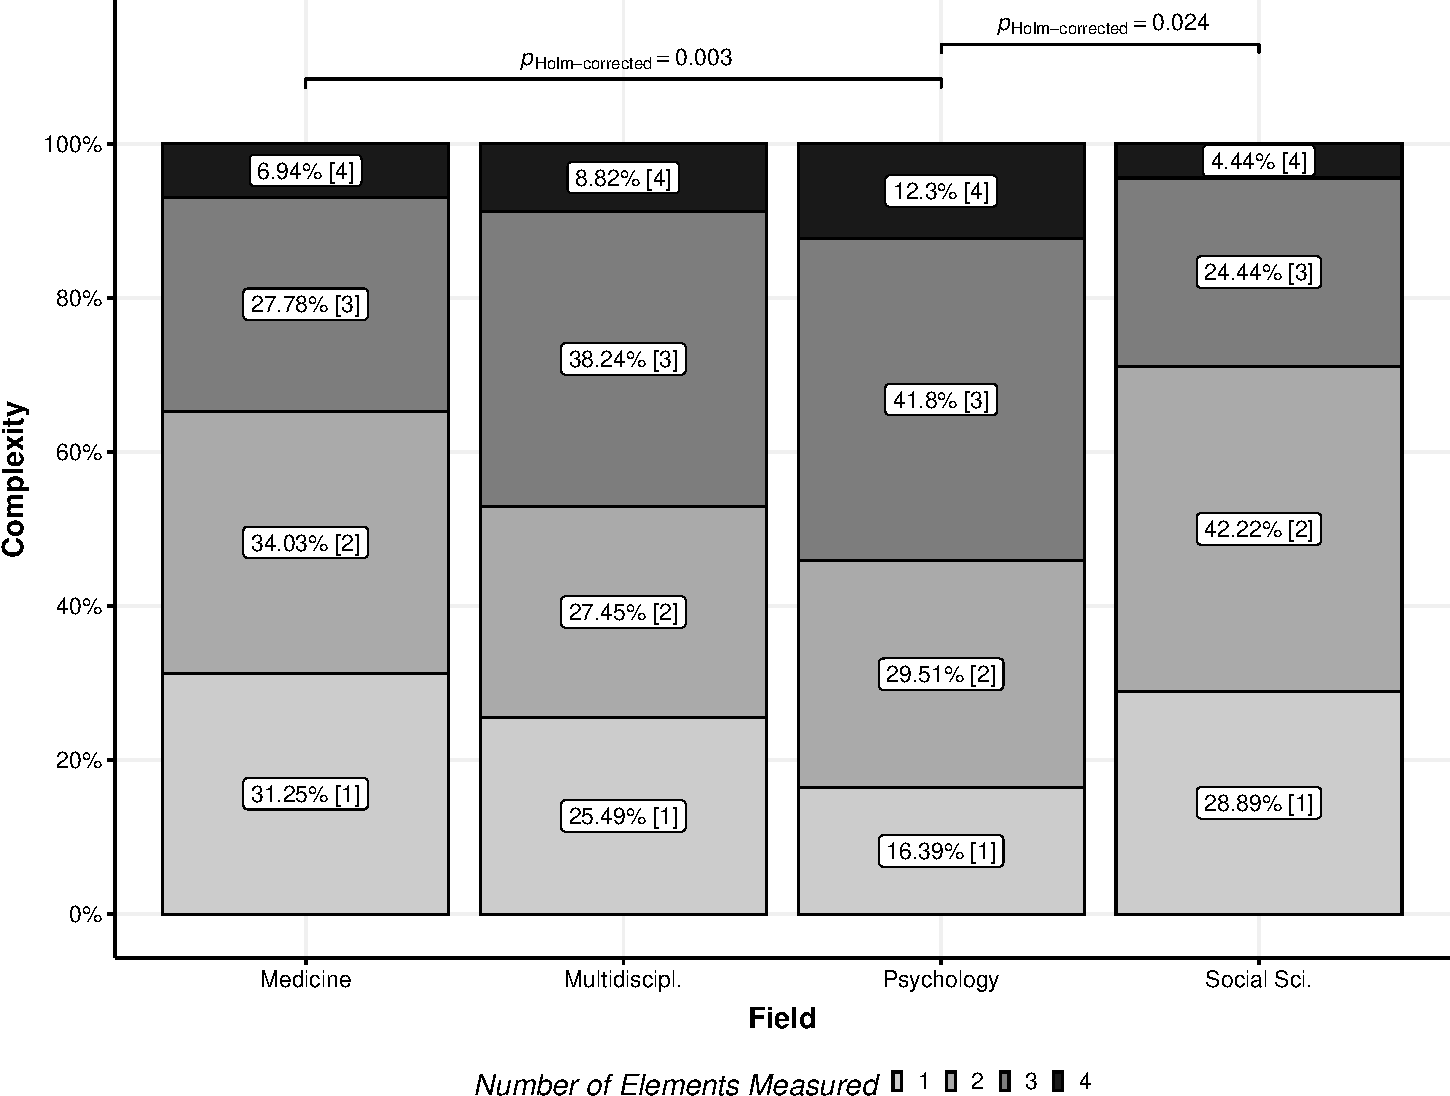
\includegraphics[width=\textwidth]{Figures/FieldPlotComplexityAverage-1}
\label{fig:FieldPlotComplexityAverage}
\end{figure}

\begin{figure}[h]
\centering
\caption{Combinations of measured experience element and their frequencies per field.}
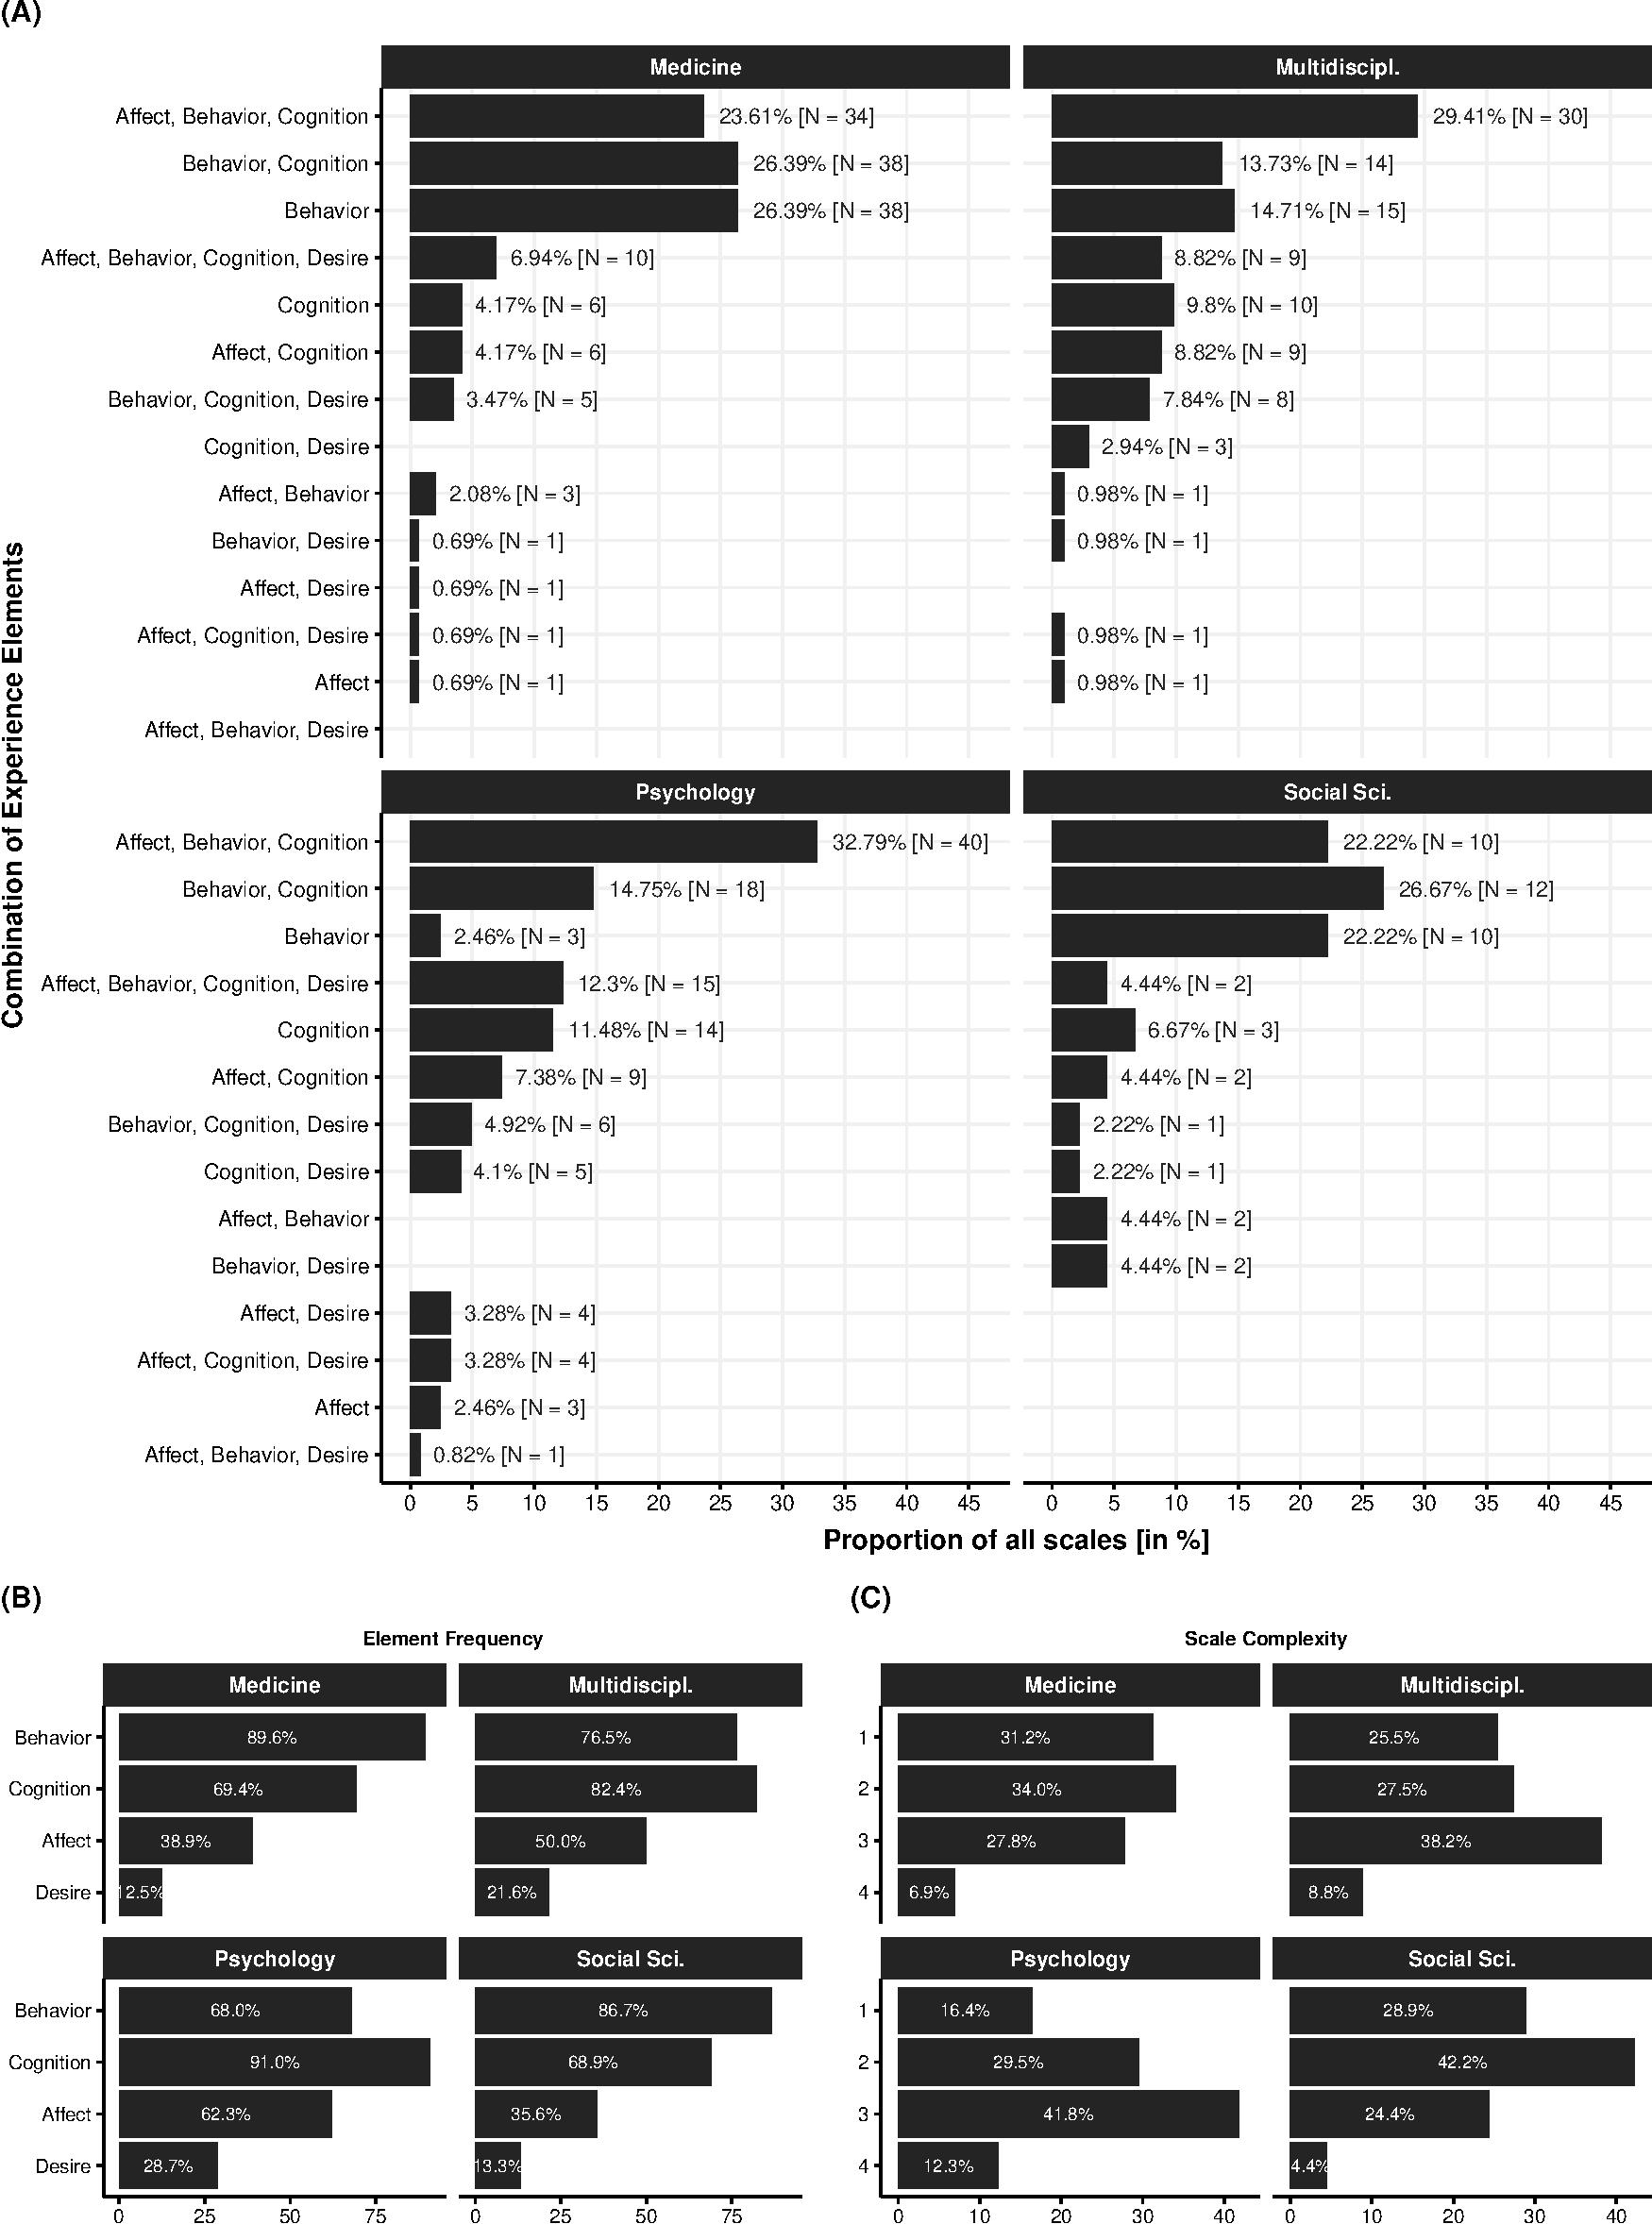
\includegraphics[width=\textwidth]{Figures/FieldPlotFreq-1}
\label{fig:FieldPlotFreq}
\end{figure}

\begin{figure}[h]
\centering
\caption{Literature Levels: Bar graph of the experience aspect frequencies for theoretical, methodological, and broader empirical literature.}
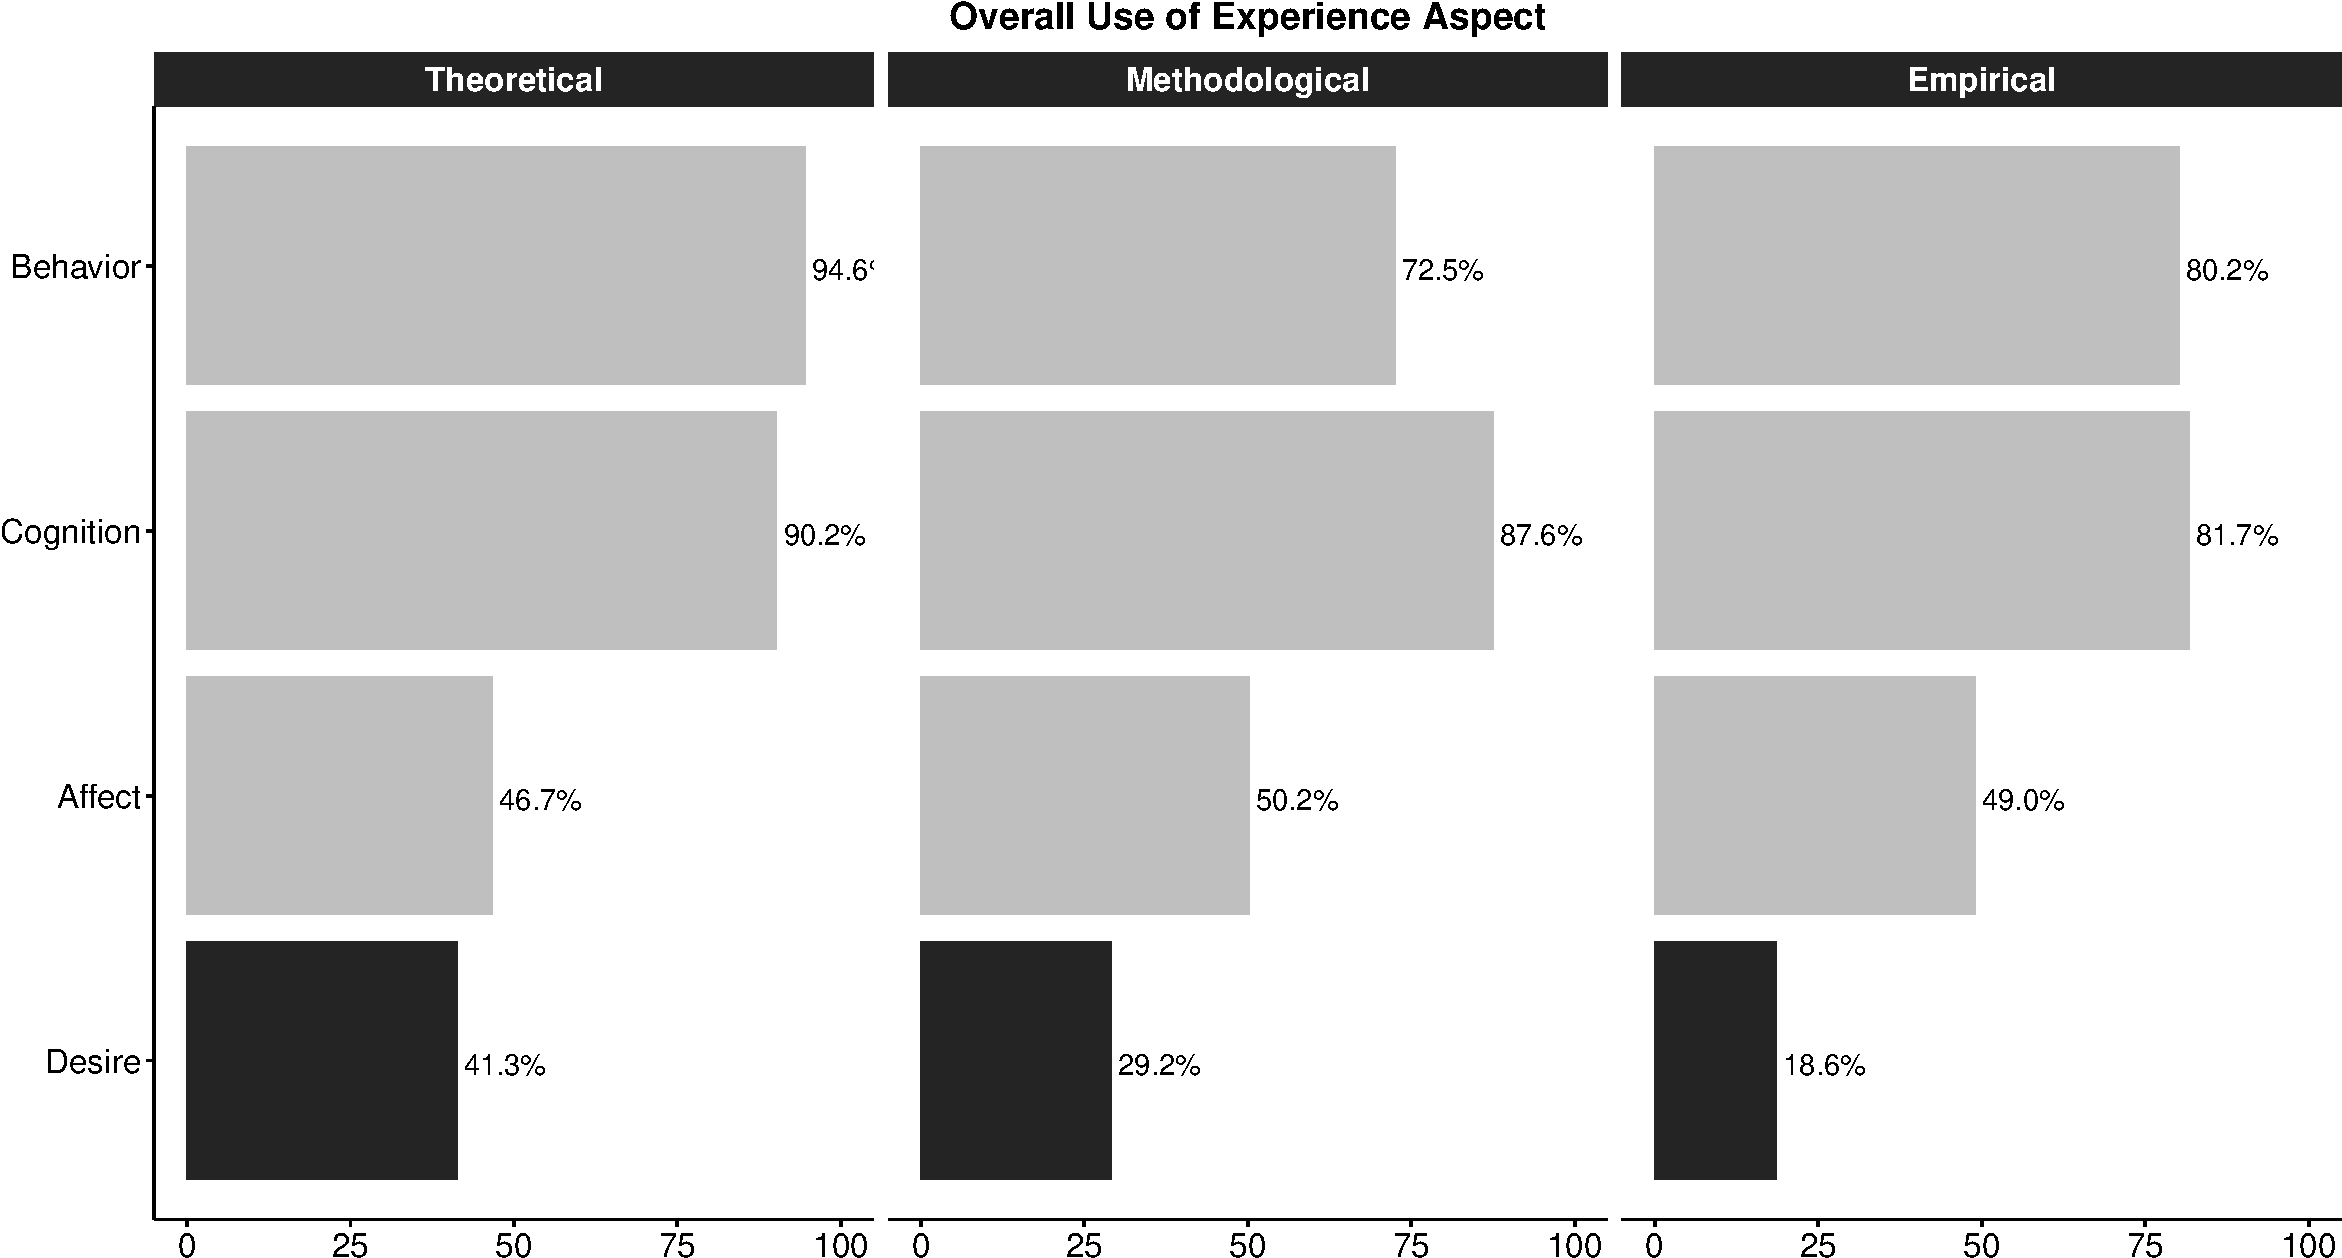
\includegraphics[width=\textwidth]{Figures/CombinedABCDBar-1}
\label{fig:CombinedAspects}
\end{figure}

\begin{figure}[h]
\centering
\caption{Literature Levels: Bar graph of the number of experience aspects used for theoretical, methodological, and broader empirical literature.}
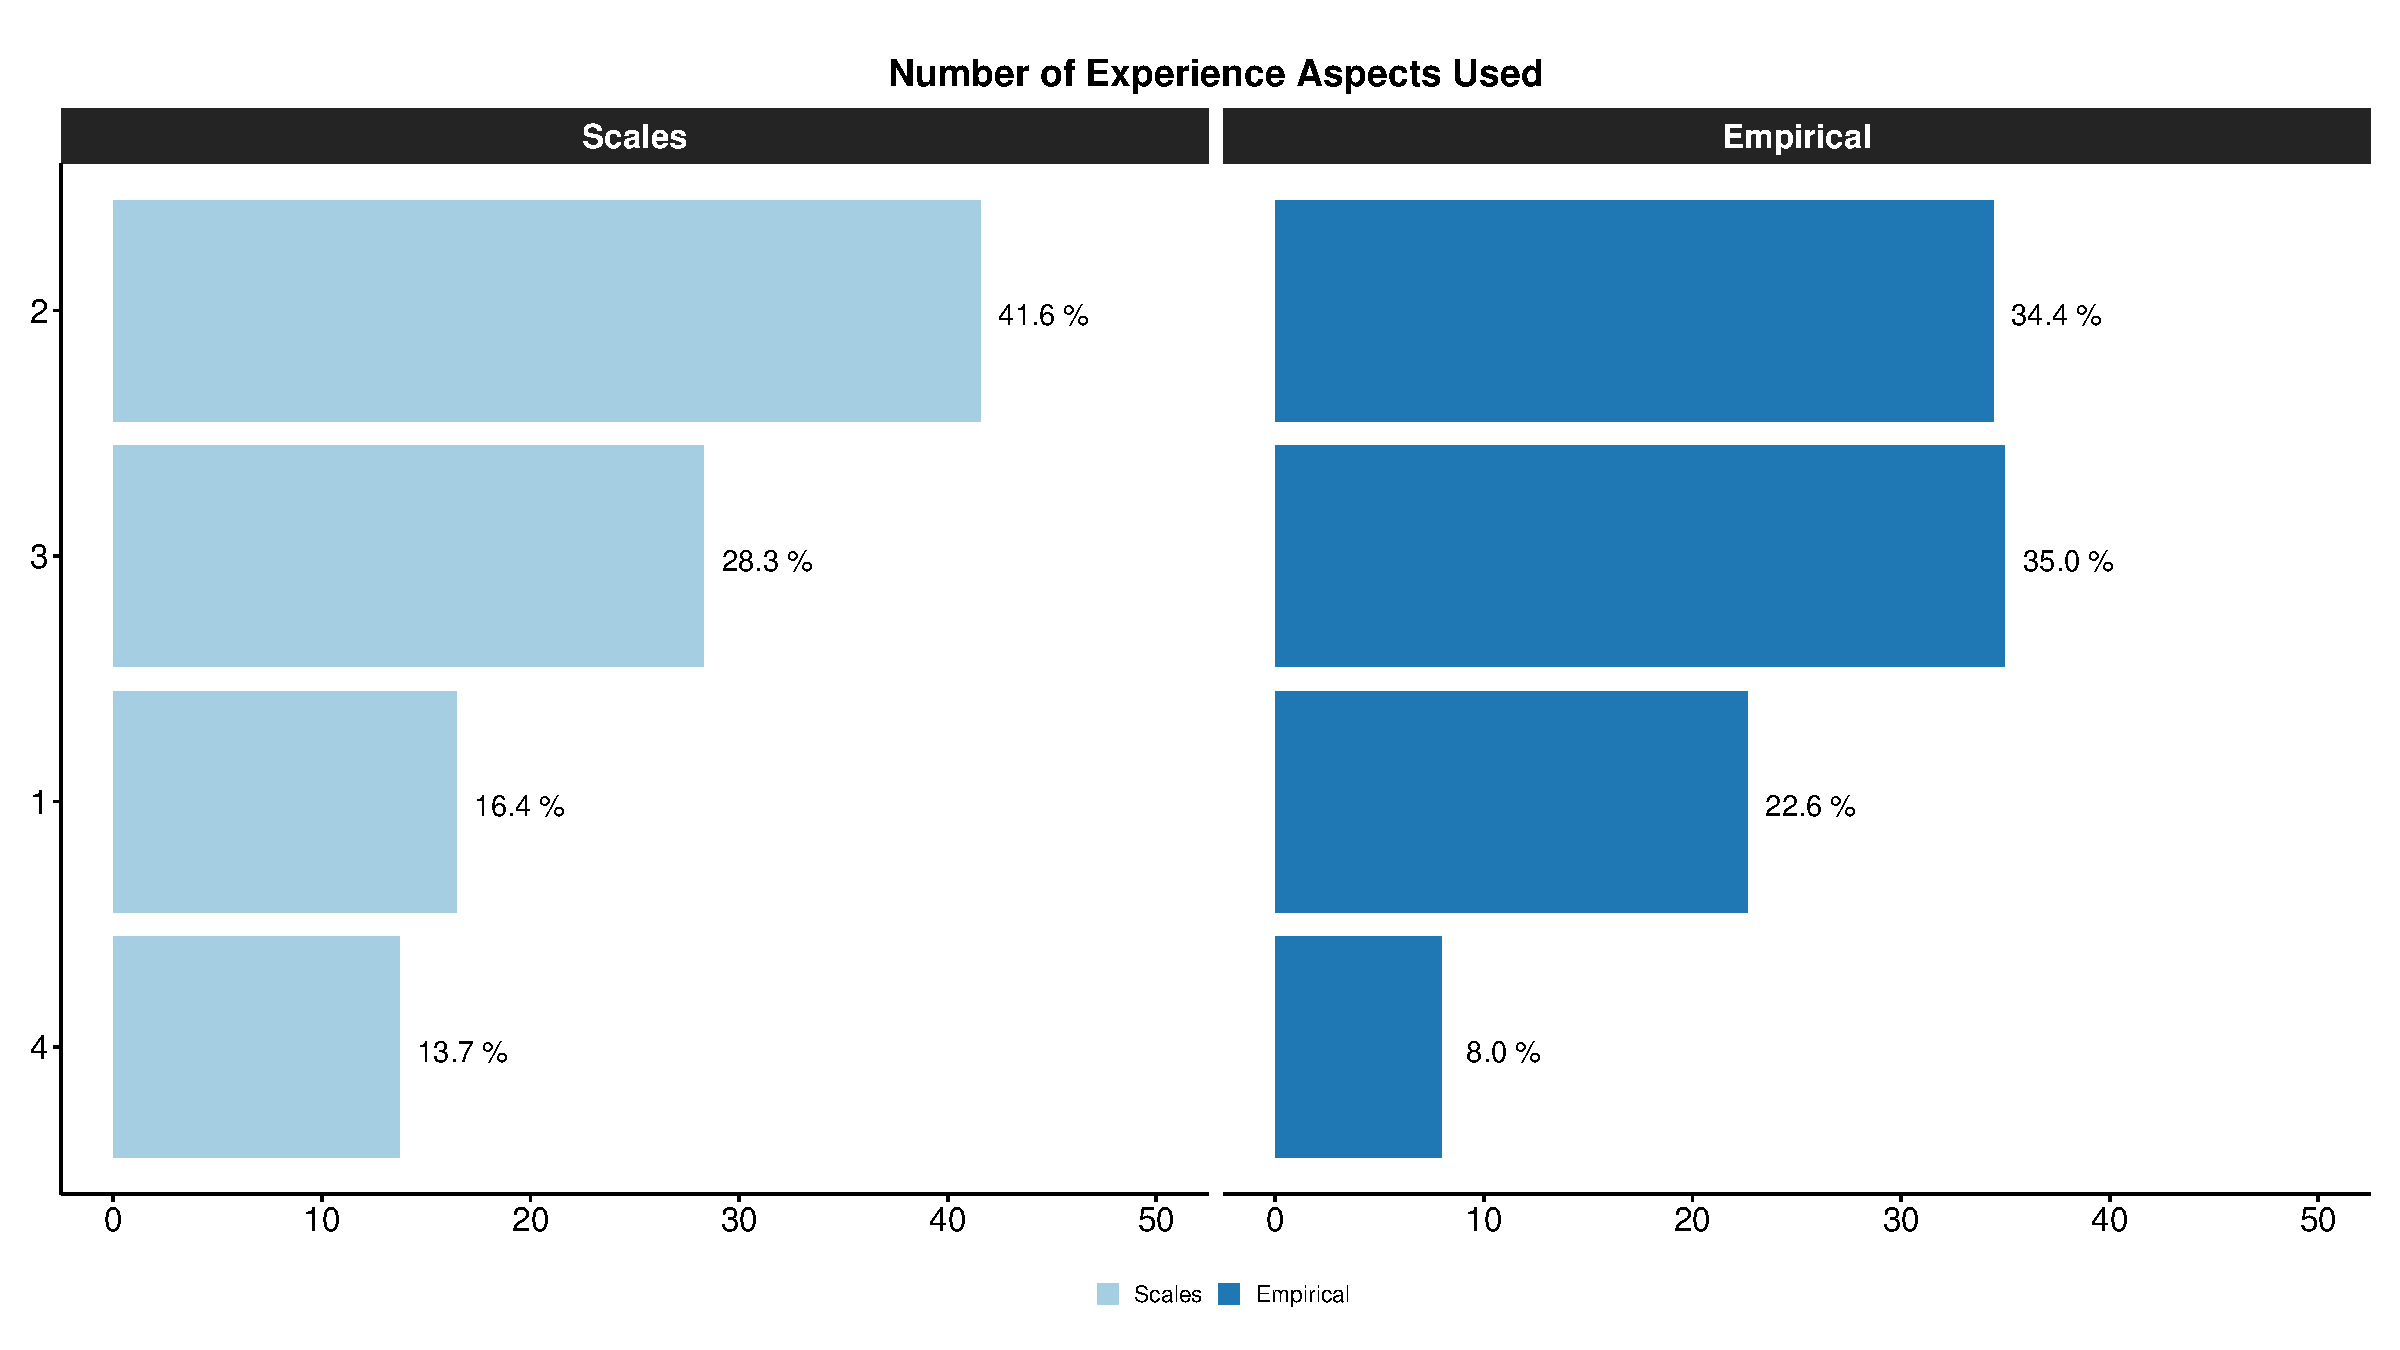
\includegraphics[width=\textwidth]{Figures/CombinedComplexityBar-1}
\label{fig:CombinedComplexity}
\end{figure}

\begin{figure}[h]
\centering
\caption{Literature Levels: Average number of additional aspects included when the aspect was considered for theoretical, methodological, and broader empirical literature [Mean ± 95\%CI].}
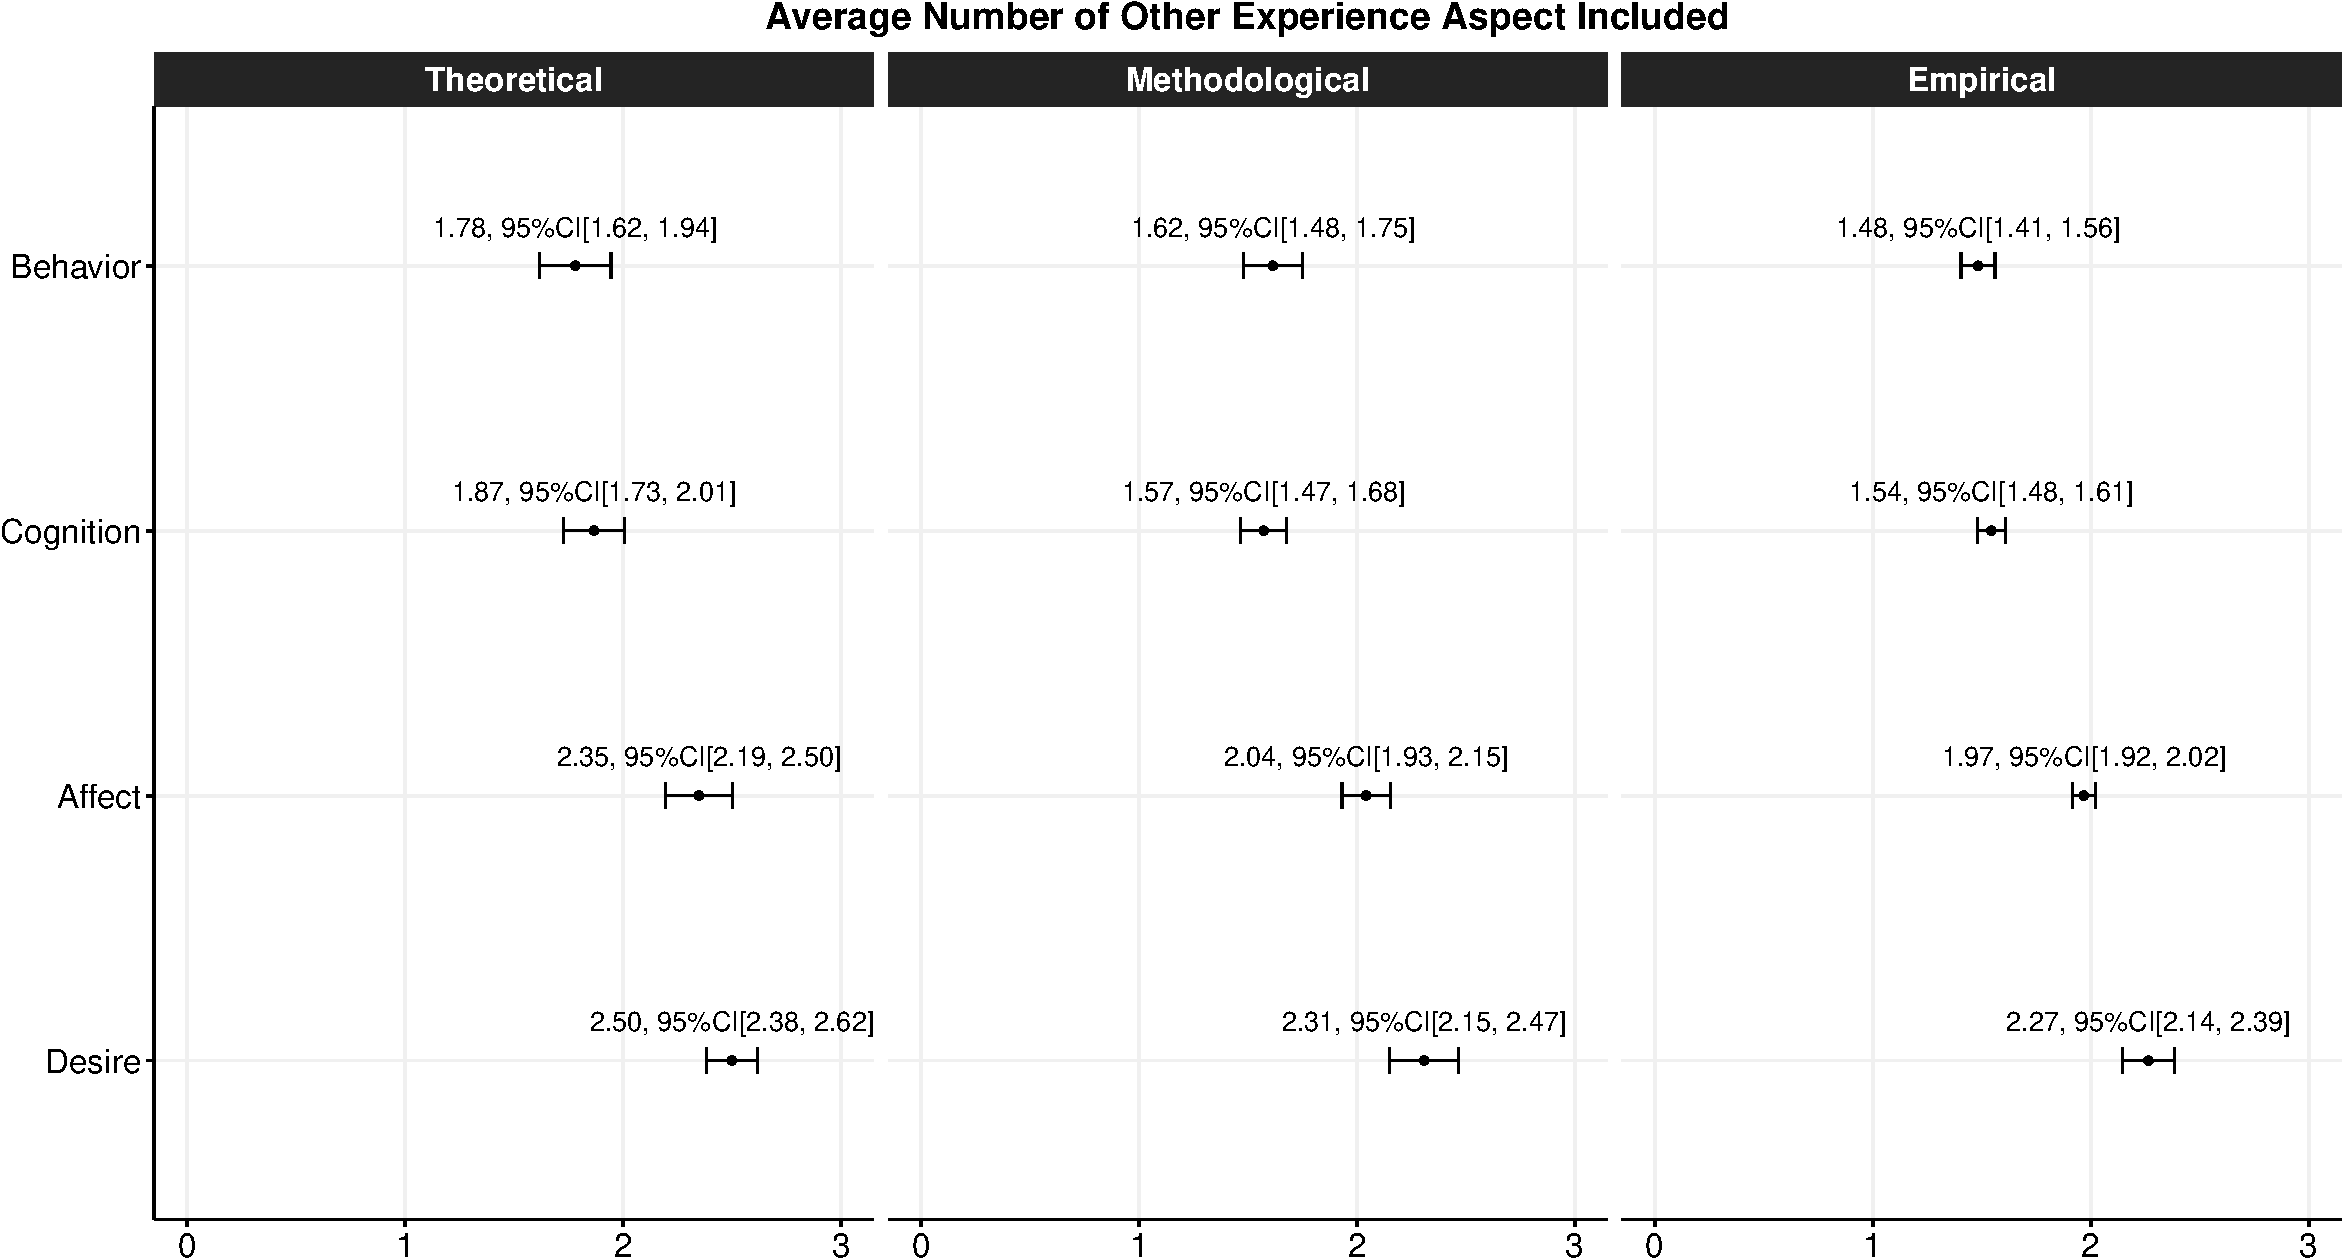
\includegraphics[width=\textwidth]{Figures/CombinedAspectComplexityMean-1}
\caption*{Note that within each literature body the aspects are not mutually exclusive (and thus not independent) because scales can include multiple experience aspects.}
\label{fig:CombinedAspectComplexity}
\end{figure}
